\documentclass{article}
\usepackage[slovak]{babel}
\usepackage[utf8]{inputenc}

\usepackage{indentfirst}
\usepackage{graphicx}

\begin{document}
    \begin{titlepage}
        \begin{center}
            \vspace{\stretch{0.382}}

            
\includegraphics[width=10cm]{FITlogo.png}\\[30mm]

            \LARGE
            Implementácia prekladača imperatívneho jazyka IFJ17 \\
            \large
            Dokumentácia k~projektu IFJ/IAL\\[55mm]

            \begin{tabular}{r l l}
                Tím: & 094 & \\
                Varianta: & II & \\
                Vedúci: & Tomáš Nereča (xnerec00) & 26\% \\
                Ďalší členovia: & Samuel Obuch (xobuch00) & 26\% \\
                    & Jiří Vozár (xvozar04) & 26\% \\
                    & Ján Farský (xfarsk00) & 22\% \\
                Implementované rozšírenia: & BASE, FUNEXP, IFTHEN &\\
            \end{tabular}

            \vspace{\stretch{0.618}}
        \end{center}
    \end{titlepage}

    \tableofcontents
    \newpage

    \section{Úvod}
        Dokumentácia popisuje implementáciu prekladača imperatívneho jazyka IFJ17. Prekladač načítava
        zdrojový kód jazyka IFJ17 zo~štandardného vstupu a ten pomocou lexikálnej, syntaktickej a sémantickej
        analýzy vyhodnotí a vygeneruje potrebné inštrukcie v~IFJcode17 pre interpret. V~prípade
        výskytu chyby pri analýze kódu IFJ17 prekladač vráti kód príslušnej chyby a chybovú hlášku na štandardný
        chybový výstup.

        Dokumentácia taktiež zahŕňa zhodnotenie práce v~tíme a približuje logiku a fungovanie
        jednotlivých častí prekladača.

    \section{Implementácia}

        \subsection{Lexikálna analýza}

        \subsection{Syntaktická analýza}
            \subsubsection{Rekurzívny zostup}
            \subsubsection{Precedenčná syntaktická analýza}

        \subsection{Tabuľka symbolov}

        \subsection{Vstavané funkcie}
            V prekladači sme implementovali aj štyri vstavané funkcie pre jazyk IFJ17 \textbf{Length, SubStr, Asc, Chr}.
            Funkcie sme implementovali ako samostatný modul. Pri ich implementovaní sme použili už definované
            inštrukcie z inštrukčnej sady, ktorá bola súčasťou jazyka IFJ17. Táto sada pracuje s premenntými v rámcoch
            s možnosťou využitia dátového zásobníku.

            \paragraph{Length, Asc a Chr}
            V inštrukčnej sade jazyka IFJ17 pre tieto tri funkcie už boli inštrukcie, ktoré vykonali spracovanie vstupov
            na požadovaný výstup. A to nasledovné: Asc - STRI2INT, Length - STRLEN, Chr - INT2CHARS
            Na nás už len bolo ošetriť iné ako ideálne prípady vstupov funkcií. Typovú kontrolu sme vzkonali už po spracovaní tokenov
            , ktoré predstavovali vstupné parametre funkcie. Hodnoty vstupov mimo povolené mädze sme ošetrili použitím iných dostupných
            inštrukcií z inštrujčnej sady.

            \paragraph{SubStr}
            Riešenie tejto funkcie bolo o niečo zložitejšie v tom, že v inštrukčnej sade nebola reišená pomocou jednej
            inštrukcie. Preto bolo potreba využiť dostupné inštrukcie a to nasledovne. Načítali sme načítali vstupné parametry
            funkcie (string a dva integery) z vrcholu zásobníku. Najprv sme sa vo vstupnom stringu posunuli na pozíciu, ktorú nám určoval
            prvý integer. Potom sme v cykle postupne čítali znak po znaku od počiatočnej pozície s využitím inštrukcie GETCHAR a lepili
            k výstupnému stringu pomocou inštrukcie CONCAT. Počet cyklov určoval druhý integer. Ošetrenie neideálnych vstupov sme
            vykonali podobne ako u predchádzajúcich vstavaných funkcií.
            
        \subsection{Generovanie kódu}

    \section{Rozšírenia}
    Boli implementované celkom 3 rozšírenia
        \begin{itemize}
            \item \textbf{base}   - podpora zadávania celočíselných konštánt v~2, 8 a 16-tkovej sústave.
            \item \textbf{funexp} - podpora volania funkcií, ktoré môžu v~argumentoch obsahovať výrazy
                                        a zároveň súčasťou výrazu môže byť volanie funkcie.
            \item  \textbf{ifthen} - podpora zjednodušenej konštrukcie podmienky If-Then bez časti Else
                                        a zároveň viacnásobnej konštrukcie Elseif-Then.
        \end{itemize}

    \section{Testovanie}
    Na začiatku sme určili jedného člena, ktorý písal jednotkové testy pre lexikálny analyzátor.
    Neskôr sme napísali zopár vlastných regresných testov.

    Keď sme sa dozvedeli o~verejnej databáze testov našich kolegov. Do nej sme prispeli aj vlastnými testami a využili ostatné testy na čo najrobustnejšie otestovanie funkčnosti nášho prekladača.

    \section{Práca v~tíme}
    Ako tím sme sa začali schádzať pomerne skoro po zaregistrovaní nášho zadania. Stretnutie sme mali
    minimálne raz týždenne, kde sme prediskutovali aktuálny stav práve implementovaných častí
    a ďalší postup či korekciu v~zdrojovom kóde. Prácu sme sa snažili rozdeľovať rovnomerne medzi
    všetkých členov tímu čo sa nie vždy darilo. Po pridelení úlohy sme stanovili deadline, aby sme
    mohli čo najskôr pokračovať na nasledujúcej časti projektu. Jednotlivé časti sme sa snažili
    implementovať paralelne s~preberanou látkou na prednáškach aby sme korektne implementovali
    jednotlivé časti a vyhli sa zbytočným chybám.

        \subsection{Správa zdrojového kódu}
        Pre správu a zdielanie zdrojových súborov sme využili verzovací systém \emph{Git} a webovú službu GitHub pre vzdialené ukladanie, ktorú sme už
        počas štúdia využili na verzovanie projektov v~iných predmetoch.

        Ako komunikačný kanál sme
        prevažne využívali skupinovú konverzáciu na sociálnej sieti Facebook, ktorá nám všetkým
        vyhovovala.

        Na sledovanie postupu pri plnení pridelených úloh a oznamovanie nájdených chýb
        sme využívali online nástroj Trello, ktorý slúži ako online kanban pre sledovanie projektov.

        Vďaka týmto informačným kanálom mohli mať všetci členovia tímu prístup k~najaktuálnejšej
        verzii projektu a reagovať na vzniknuté chyby efektívne.

        \newpage
        \subsection{Rozdelenie}
        \noindent
        Bodové rozdelenie je nasledovné:\\~\\
        \begin{tabular}{l l}
            Tomáš Nereča (xnerec00) & 26\% \\
            Samuel Obuch (xobuch00) & 26\% \\
            Jiří Vozár (xvozar04)   & 26\% \\
            Ján Farský (xfarsk00)   & 22\% \\
        \end{tabular} \\
        Dôvod nerovnomerného rozdelenia bodov bolo nedostatočné splnenie pridelených častí jednému
        z~členov tímu, čo viedlo k~potrebnému prepisu zdrojového kódu ostatnými členmi tímu.

    \section{Záver}
    S~projektom podobného rozsahu sa ešte nikto z~nás predtým nestretol, preto ho pokladáme za dobrú
    skúsenosť pre každého z~nás. Pri jeho riešení sme prakticky využili získané vedomosti z~predmetov
    IFJ a IAL.

    Pre správne fungovanie tímu bola potrebná dobrá komunikácia, riadenie a pridelovanie úloh, ktoré pretvali počas celého
    priebehu projektu či už vďaka pravidelným stretnutiam alebo využitým nástrojom ale aj individuálne
    schopnosti jednotlivých členov. Výsledkom tejto práce je funkčný a z~nášho pohľadu vydarený
    prekladač jazyka IFJ17.

    \newpage
    \section{Prílohy}
        \subsection{Diagram konečného automatu}
            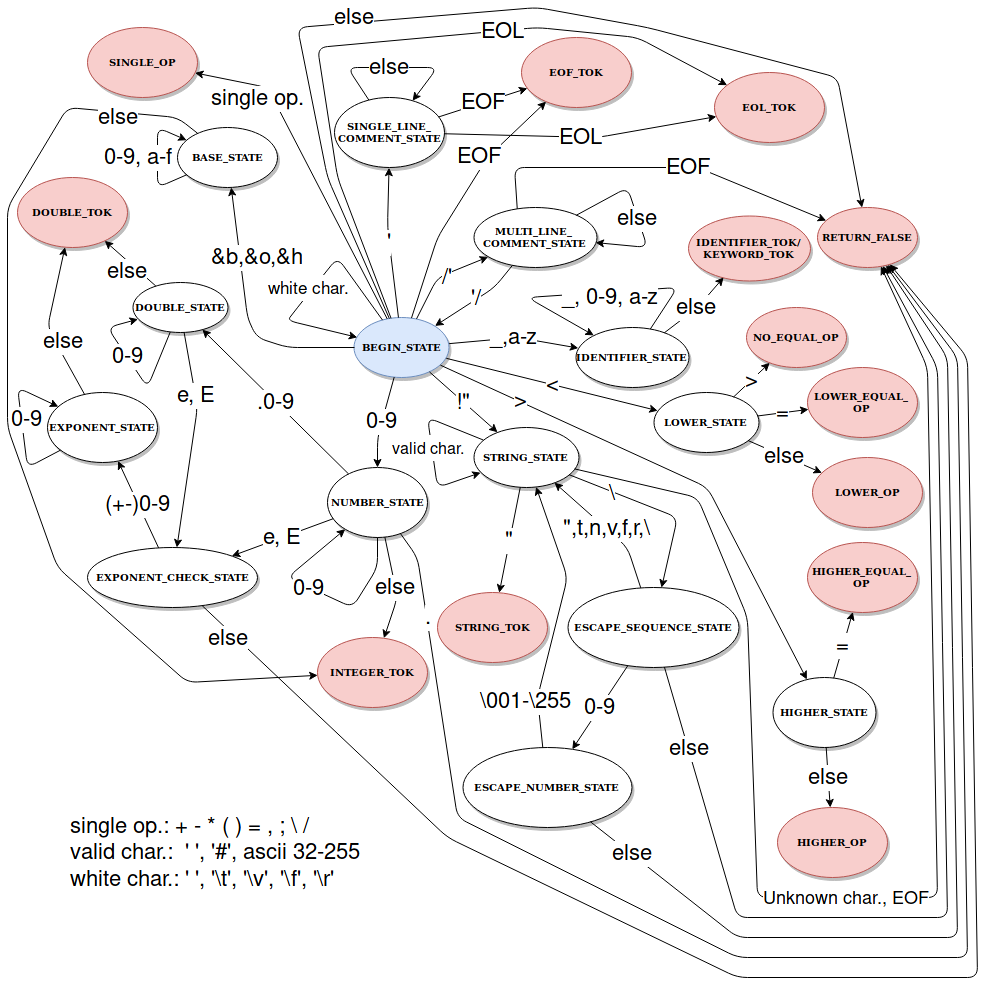
\includegraphics[trim=6cm 0 0 0, width=15cm]{finite_automata.png}
        \subsection{LL gramatika}
        \subsection{LL tabuľka}
        \subsection{Precedenčná tabuľka}

\end{document}
